\documentclass[11pt]{article}
\usepackage[margin=1in]{geometry}
\usepackage{graphicx}
\usepackage{float}
\usepackage{caption}
\captionsetup{font=small, labelfont=bf}

\title{Lab 2: Transformers for In-Context Regression}
\author{Chris Sellgren}
\date{}

\begin{document}
\maketitle

\section*{The data}

\begin{figure}[H]
  \centering
  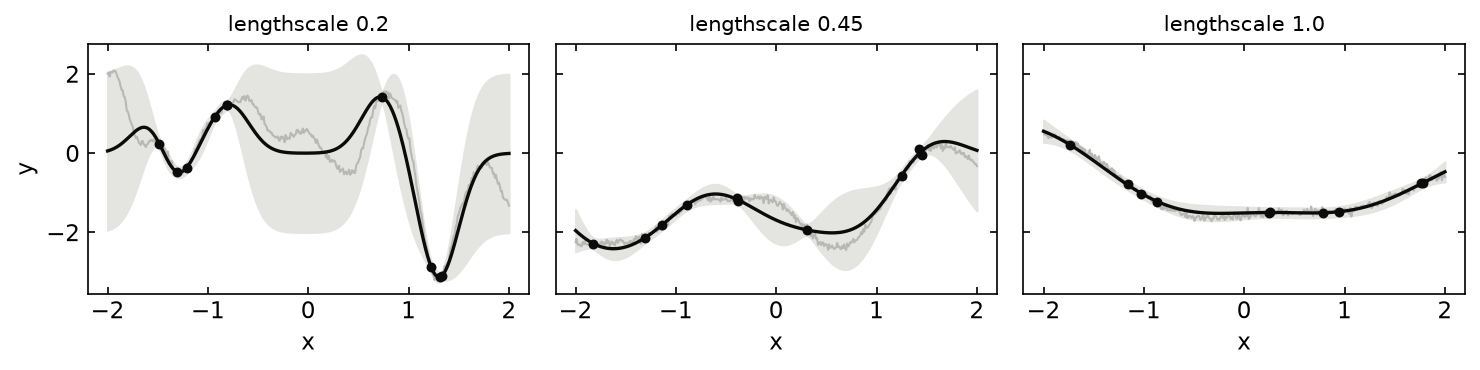
\includegraphics[width=\linewidth]{figures/gp_examples.png}
  \caption{Example functions drawn from the Gaussian process at three lengthscales, with 10 noisy context
  points (black), the true function (light gray), and the exact GP posterior mean $\pm 2\sigma$.}
\end{figure}

\section*{Transformer}

\begin{figure}[H]
  \centering
  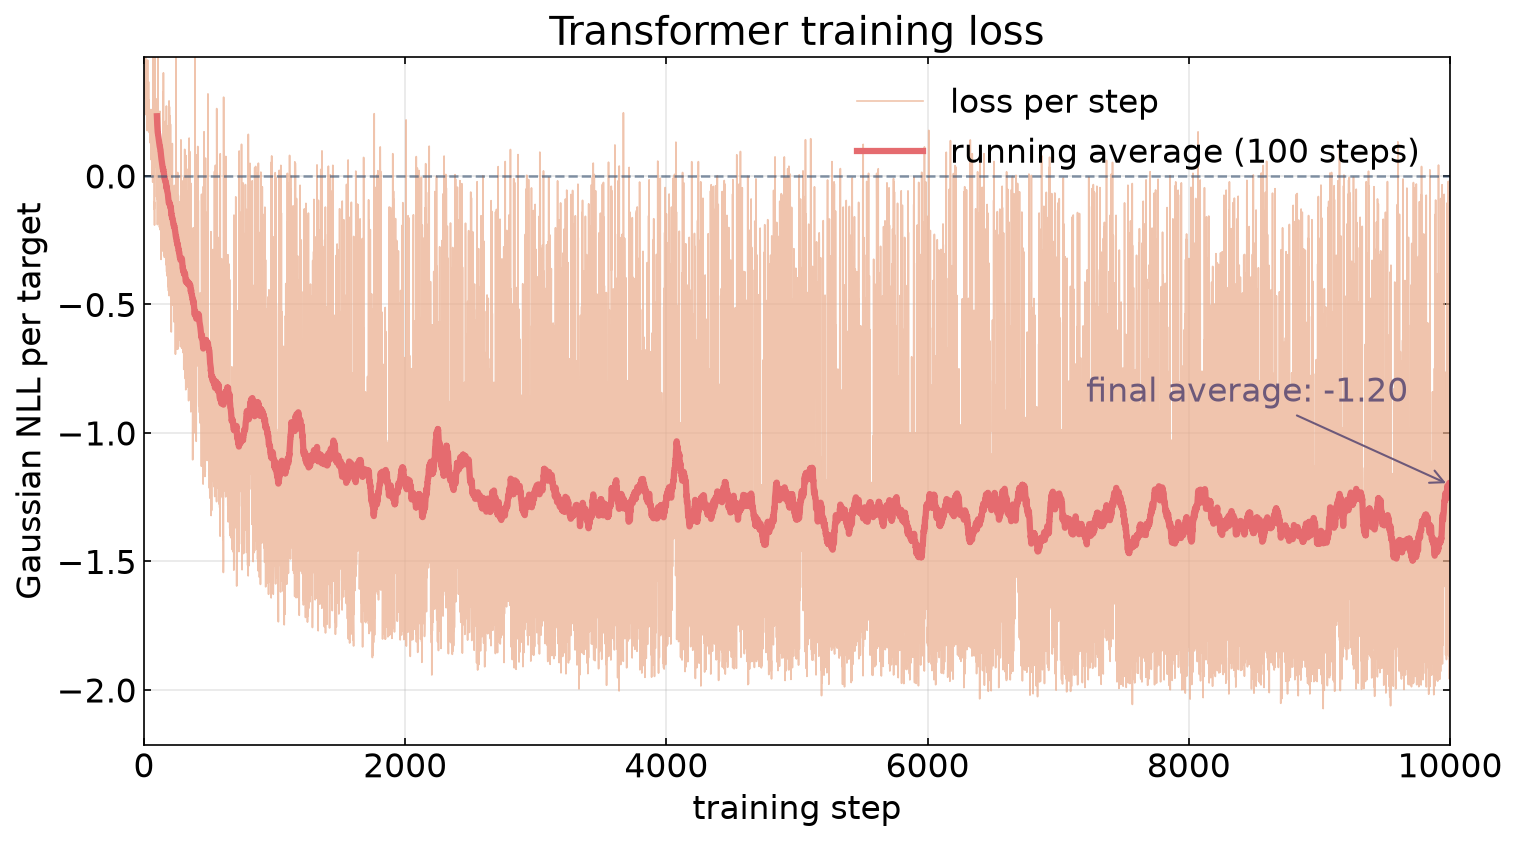
\includegraphics[width=0.85\linewidth]{figures/transformer_loss.png}
  \caption{Transformer training loss (Gaussian NLL per target) per step, with a 100-step running average.}
\end{figure}

\begin{figure}[H]
  \centering
  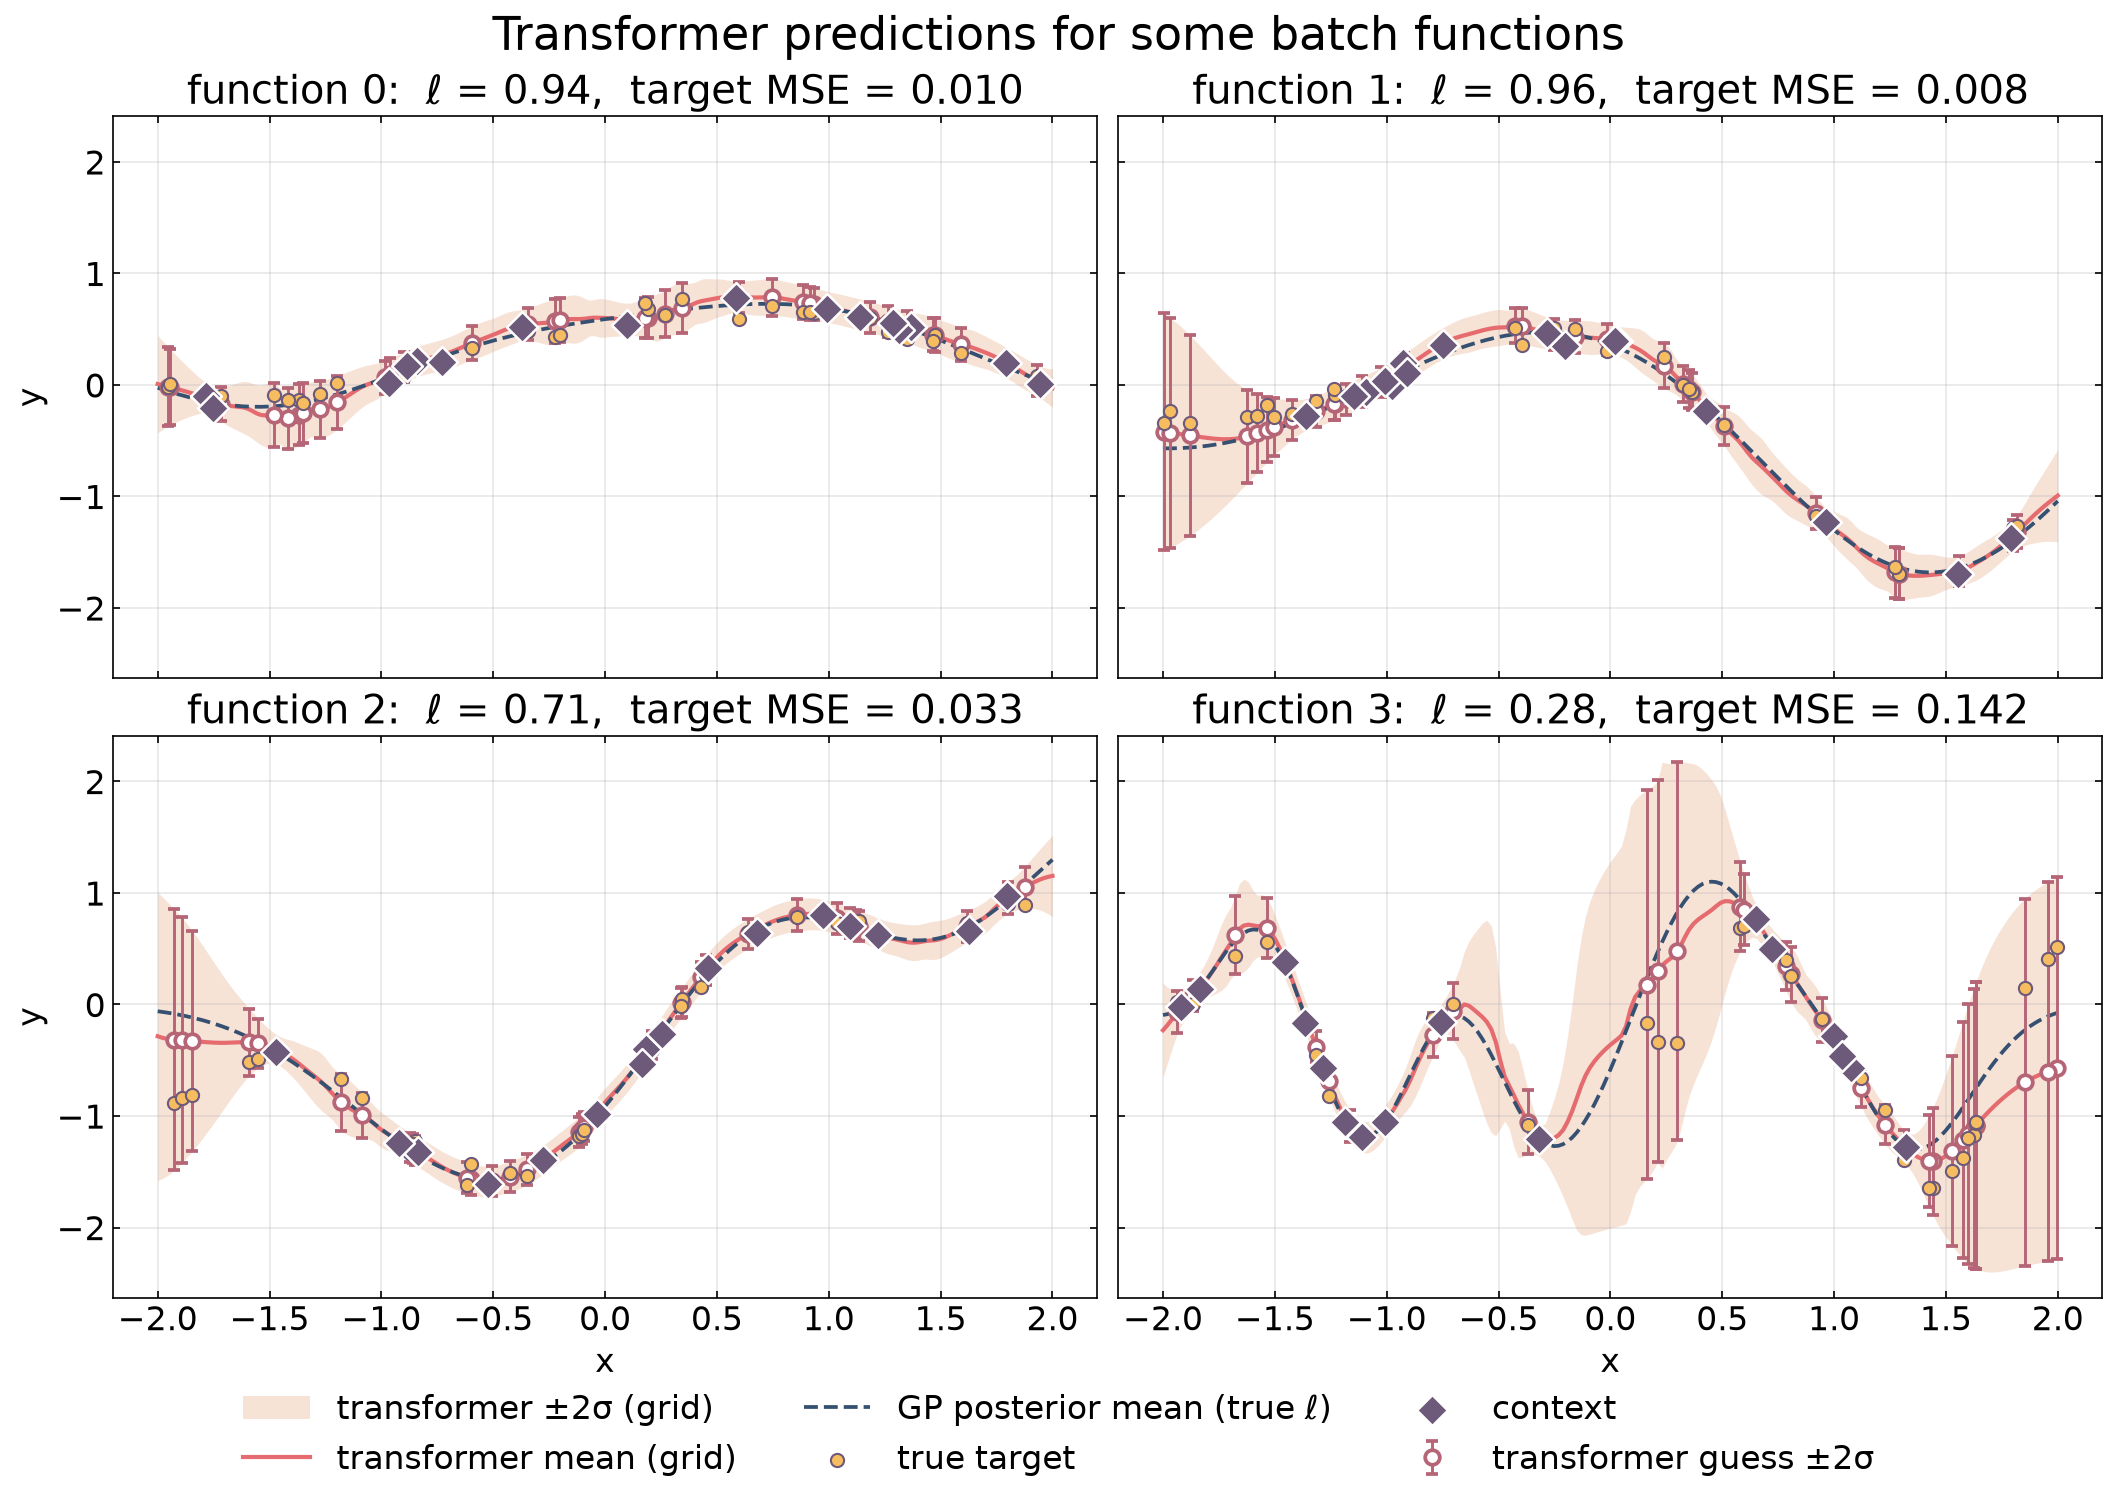
\includegraphics[width=0.9\linewidth]{figures/transformer_predictions.png}
  \caption{Transformer predictions for four functions: guesses at the target points with $\pm 2\sigma$ error
  bars, the prediction on a dense grid, the true targets, the context, and the exact GP posterior mean.}
\end{figure}

\begin{figure}[H]
  \centering
  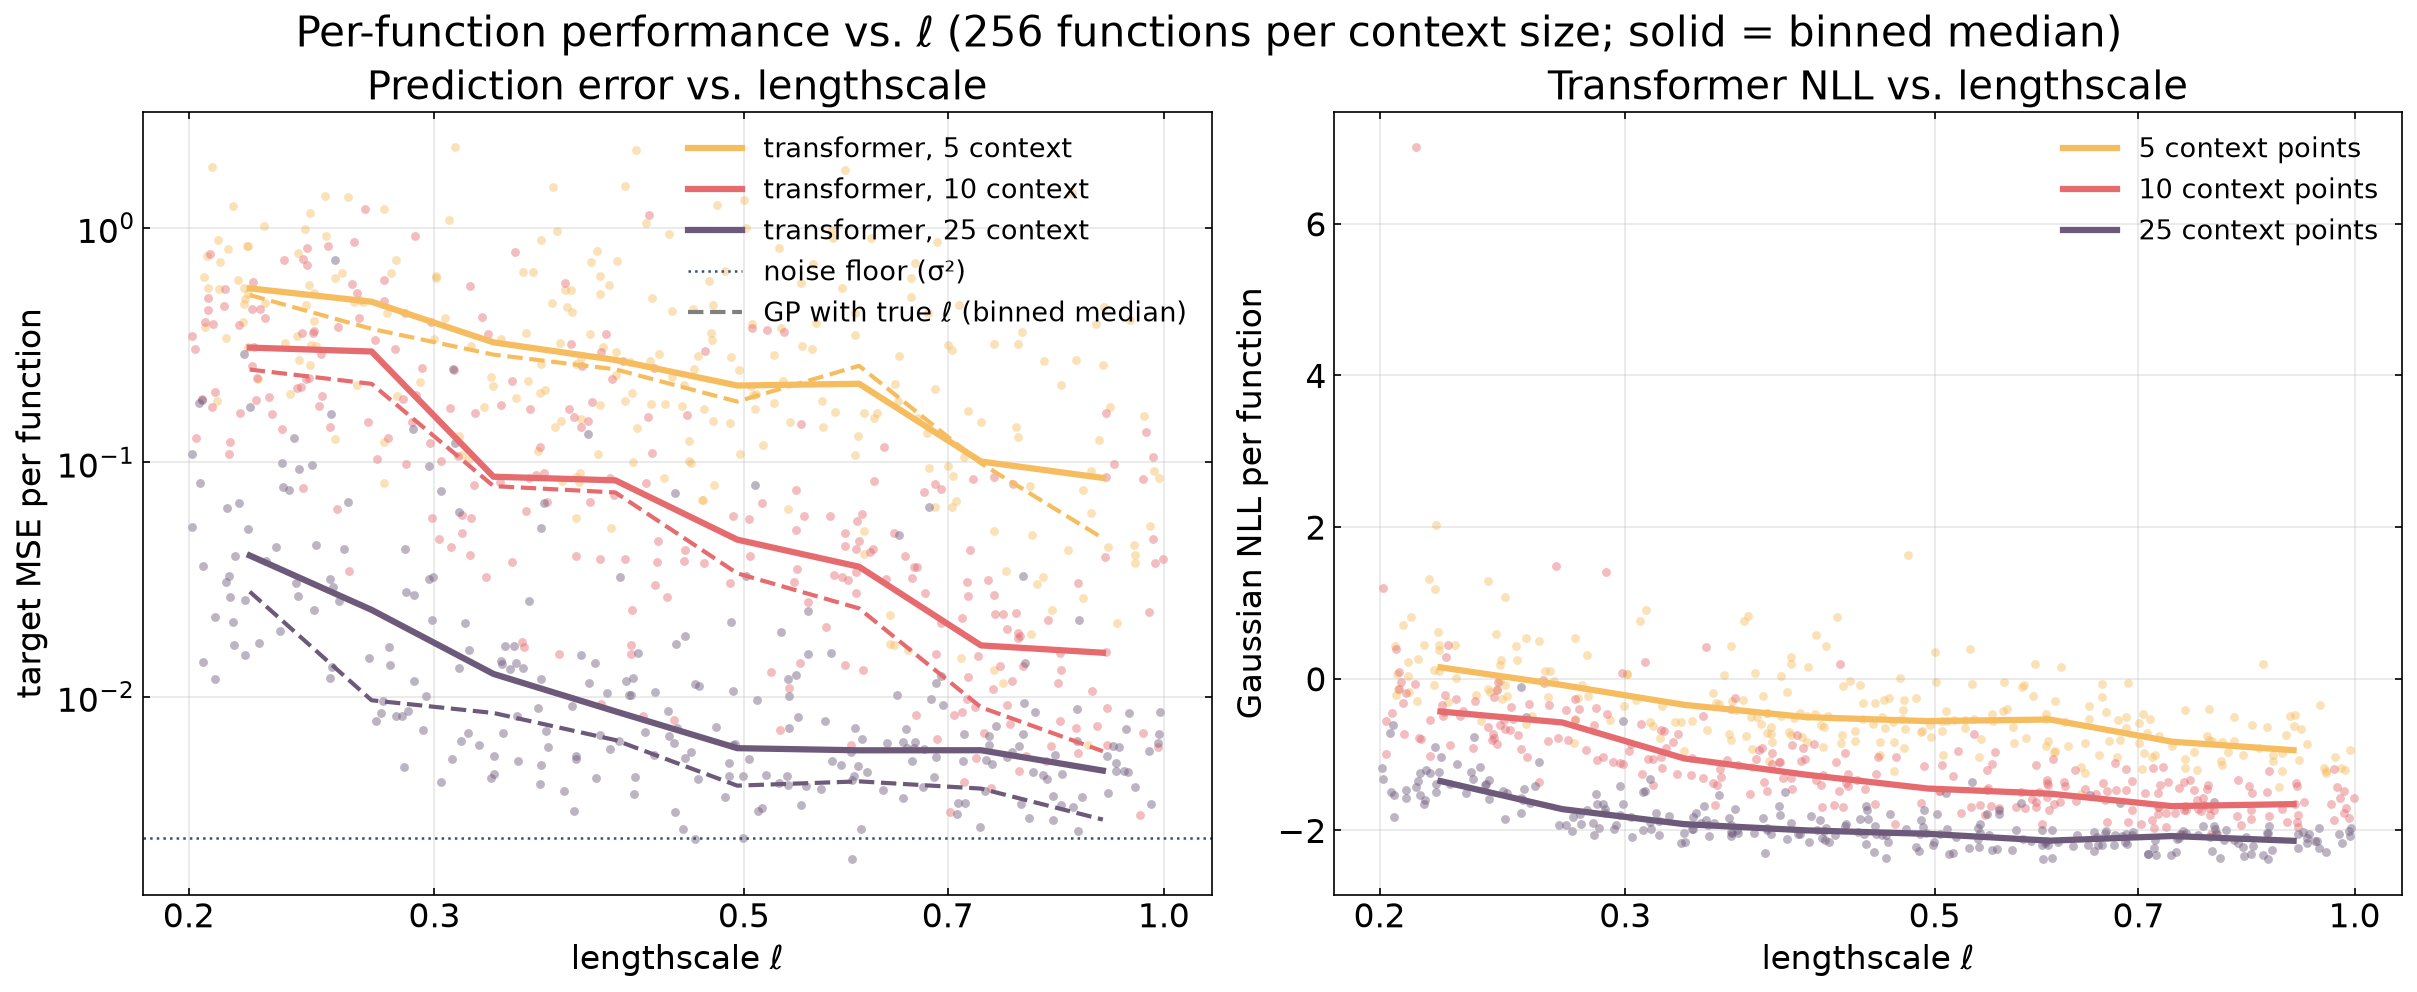
\includegraphics[width=\linewidth]{figures/performance_vs_lengthscale.png}
  \caption{Per-function transformer error (left, with the GP for comparison) and NLL (right) against the
  lengthscale $\ell$, for 5, 10 and 25 context points.}
\end{figure}

\section*{MLP comparison}

\begin{figure}[H]
  \centering
  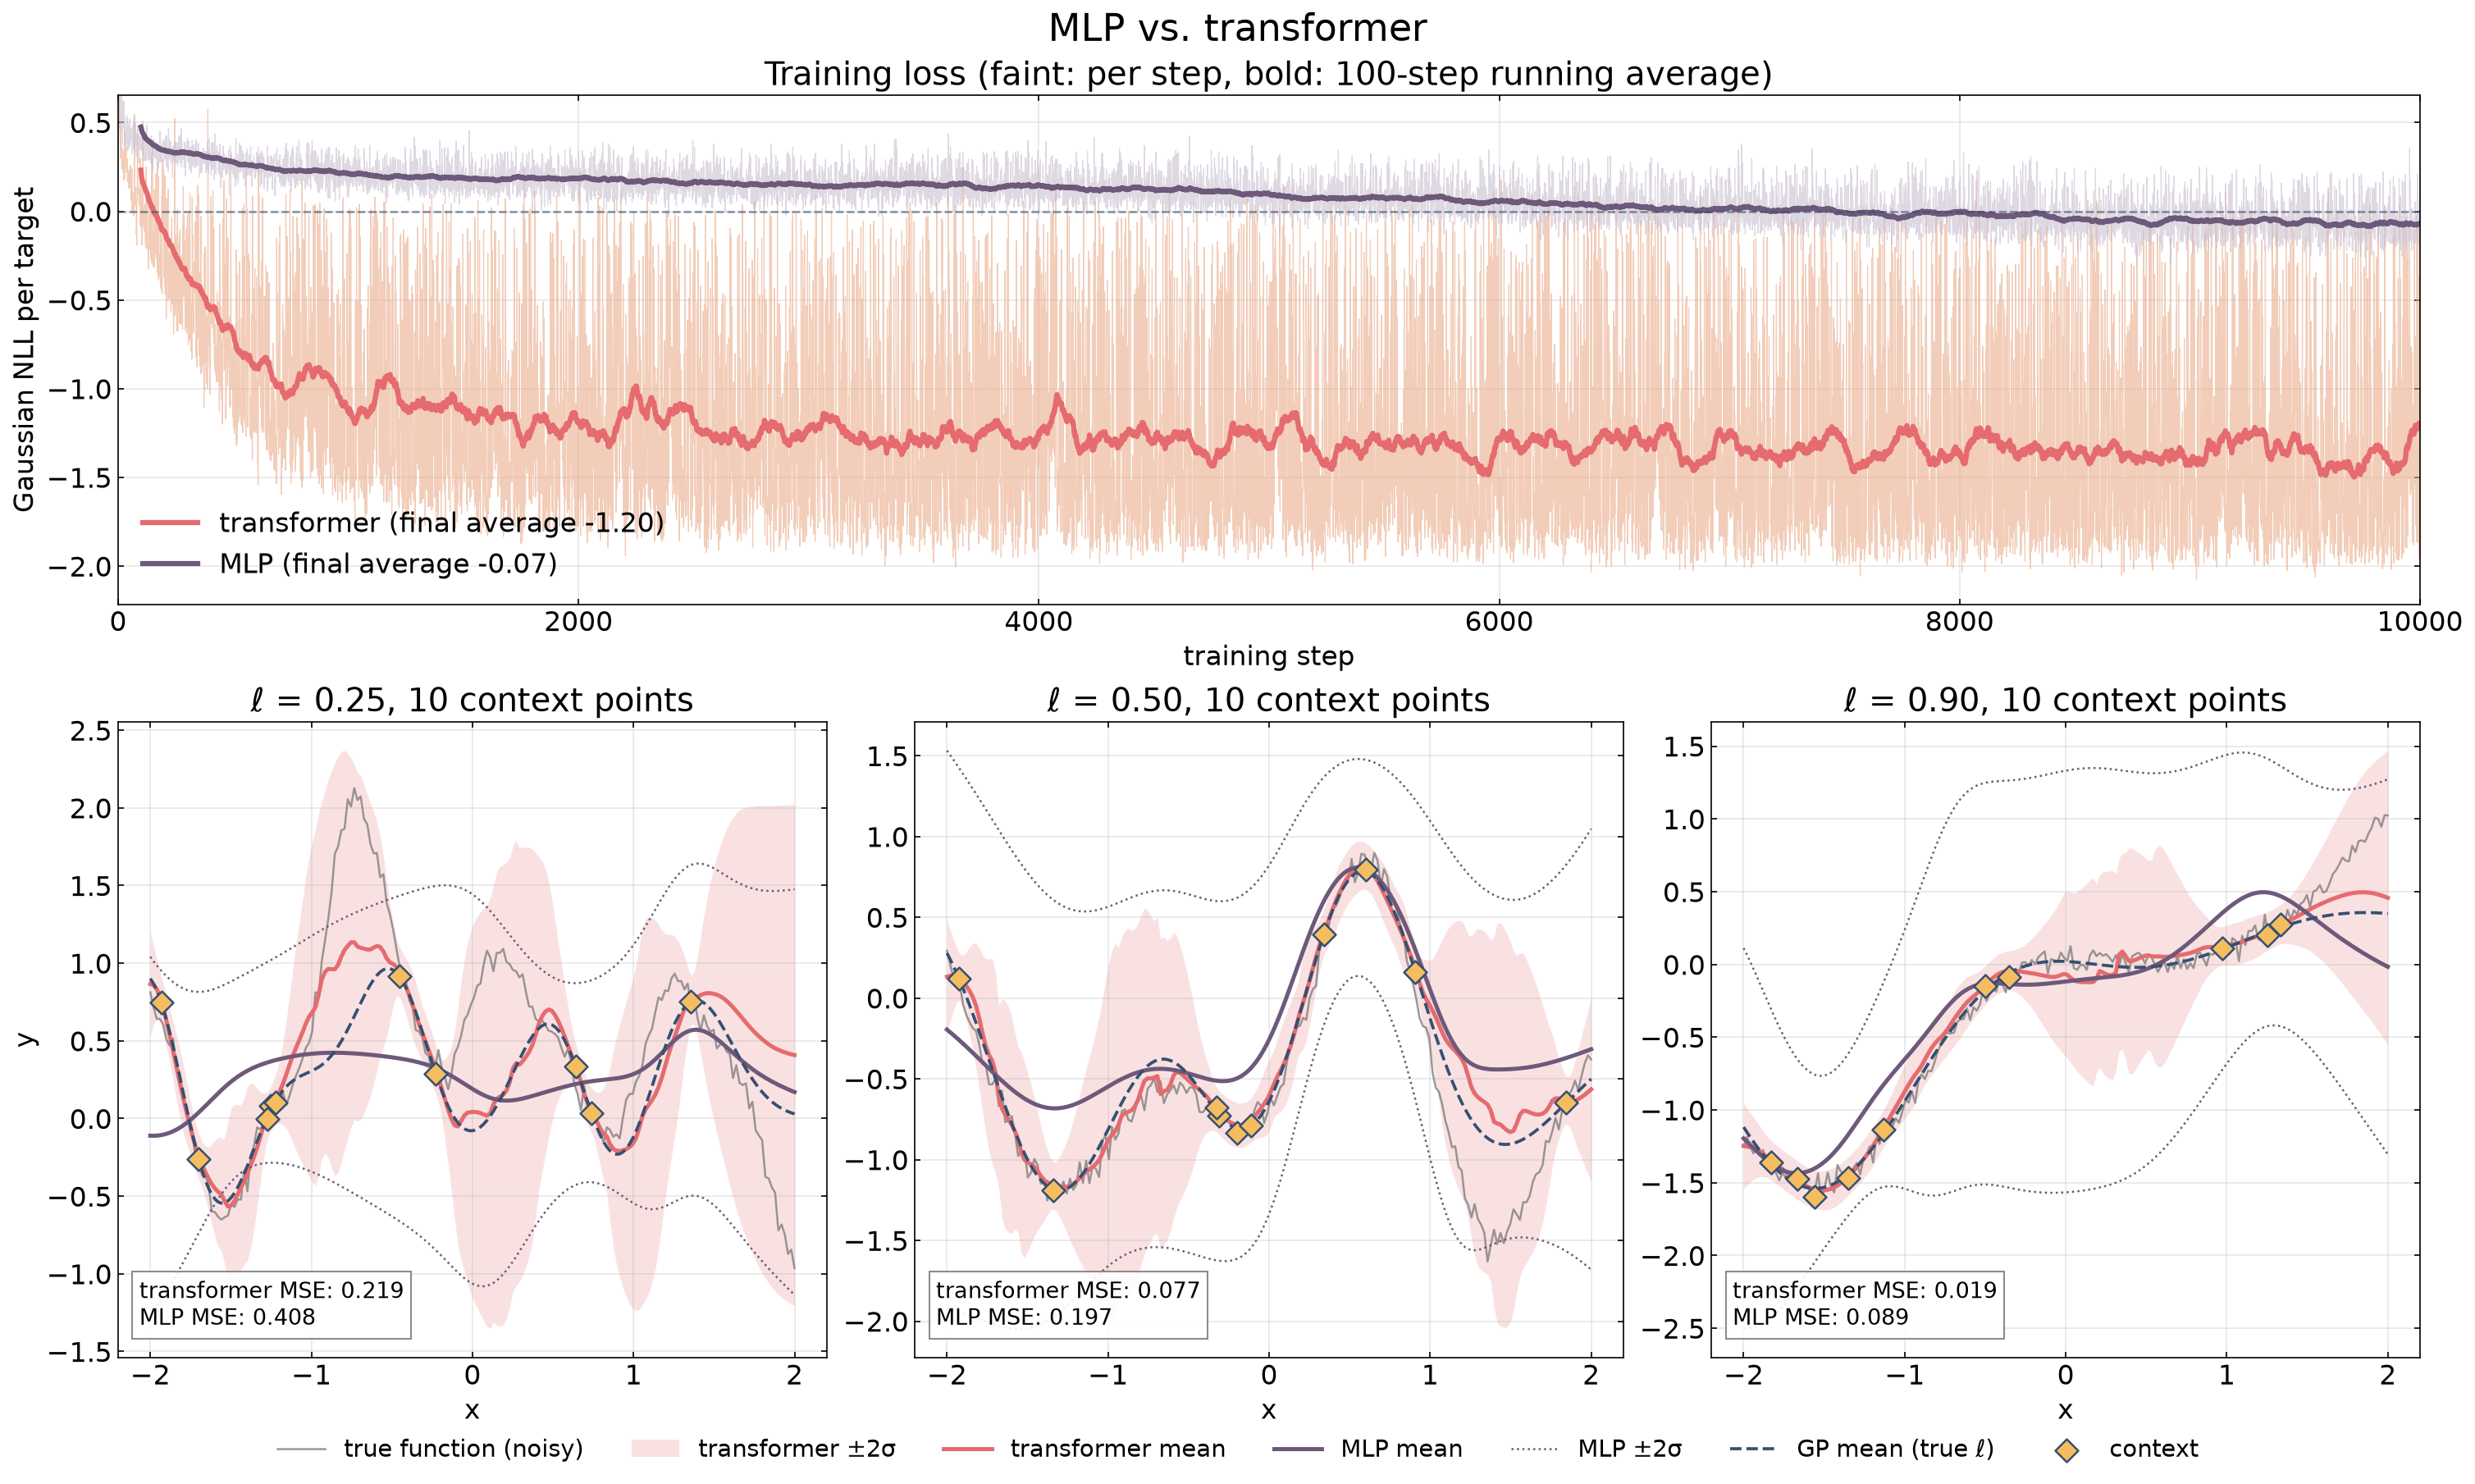
\includegraphics[width=\linewidth]{figures/mlp_comparison.png}
  \caption{MLP vs.\ transformer: training loss of both models (top), and both models' predictions with
  $\pm 2\sigma$ on three functions with short, medium and long lengthscales (bottom).}
\end{figure}

\section*{Results}

\begin{figure}[H]
  \centering
  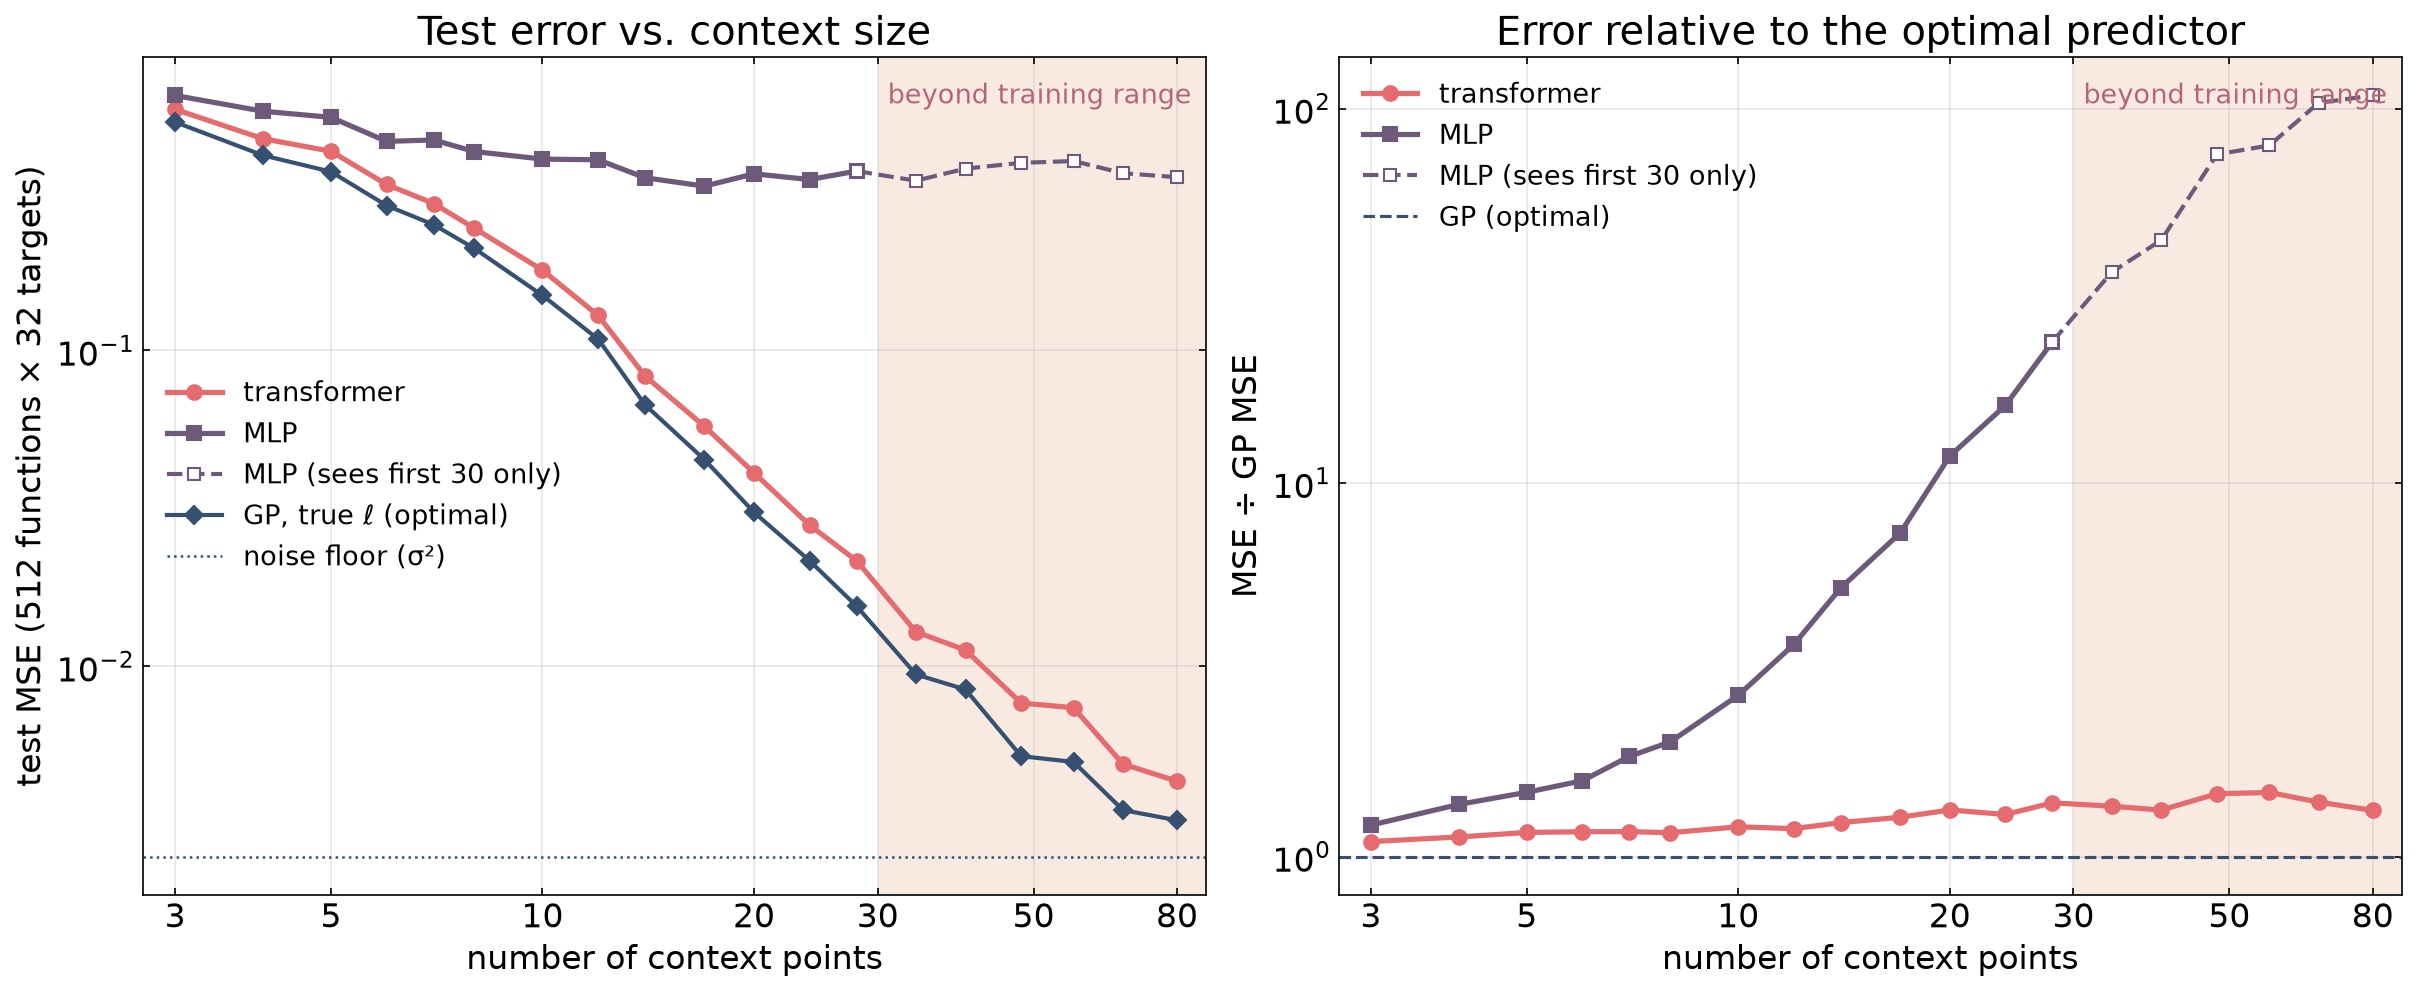
\includegraphics[width=\linewidth]{figures/error_vs_context.png}
  \caption{Test error against the number of context points (3 to 80) for the transformer, the MLP and the
  GP with the true lengthscale (left), and each model's error relative to the GP (right).}
\end{figure}

\begin{figure}[H]
  \centering
  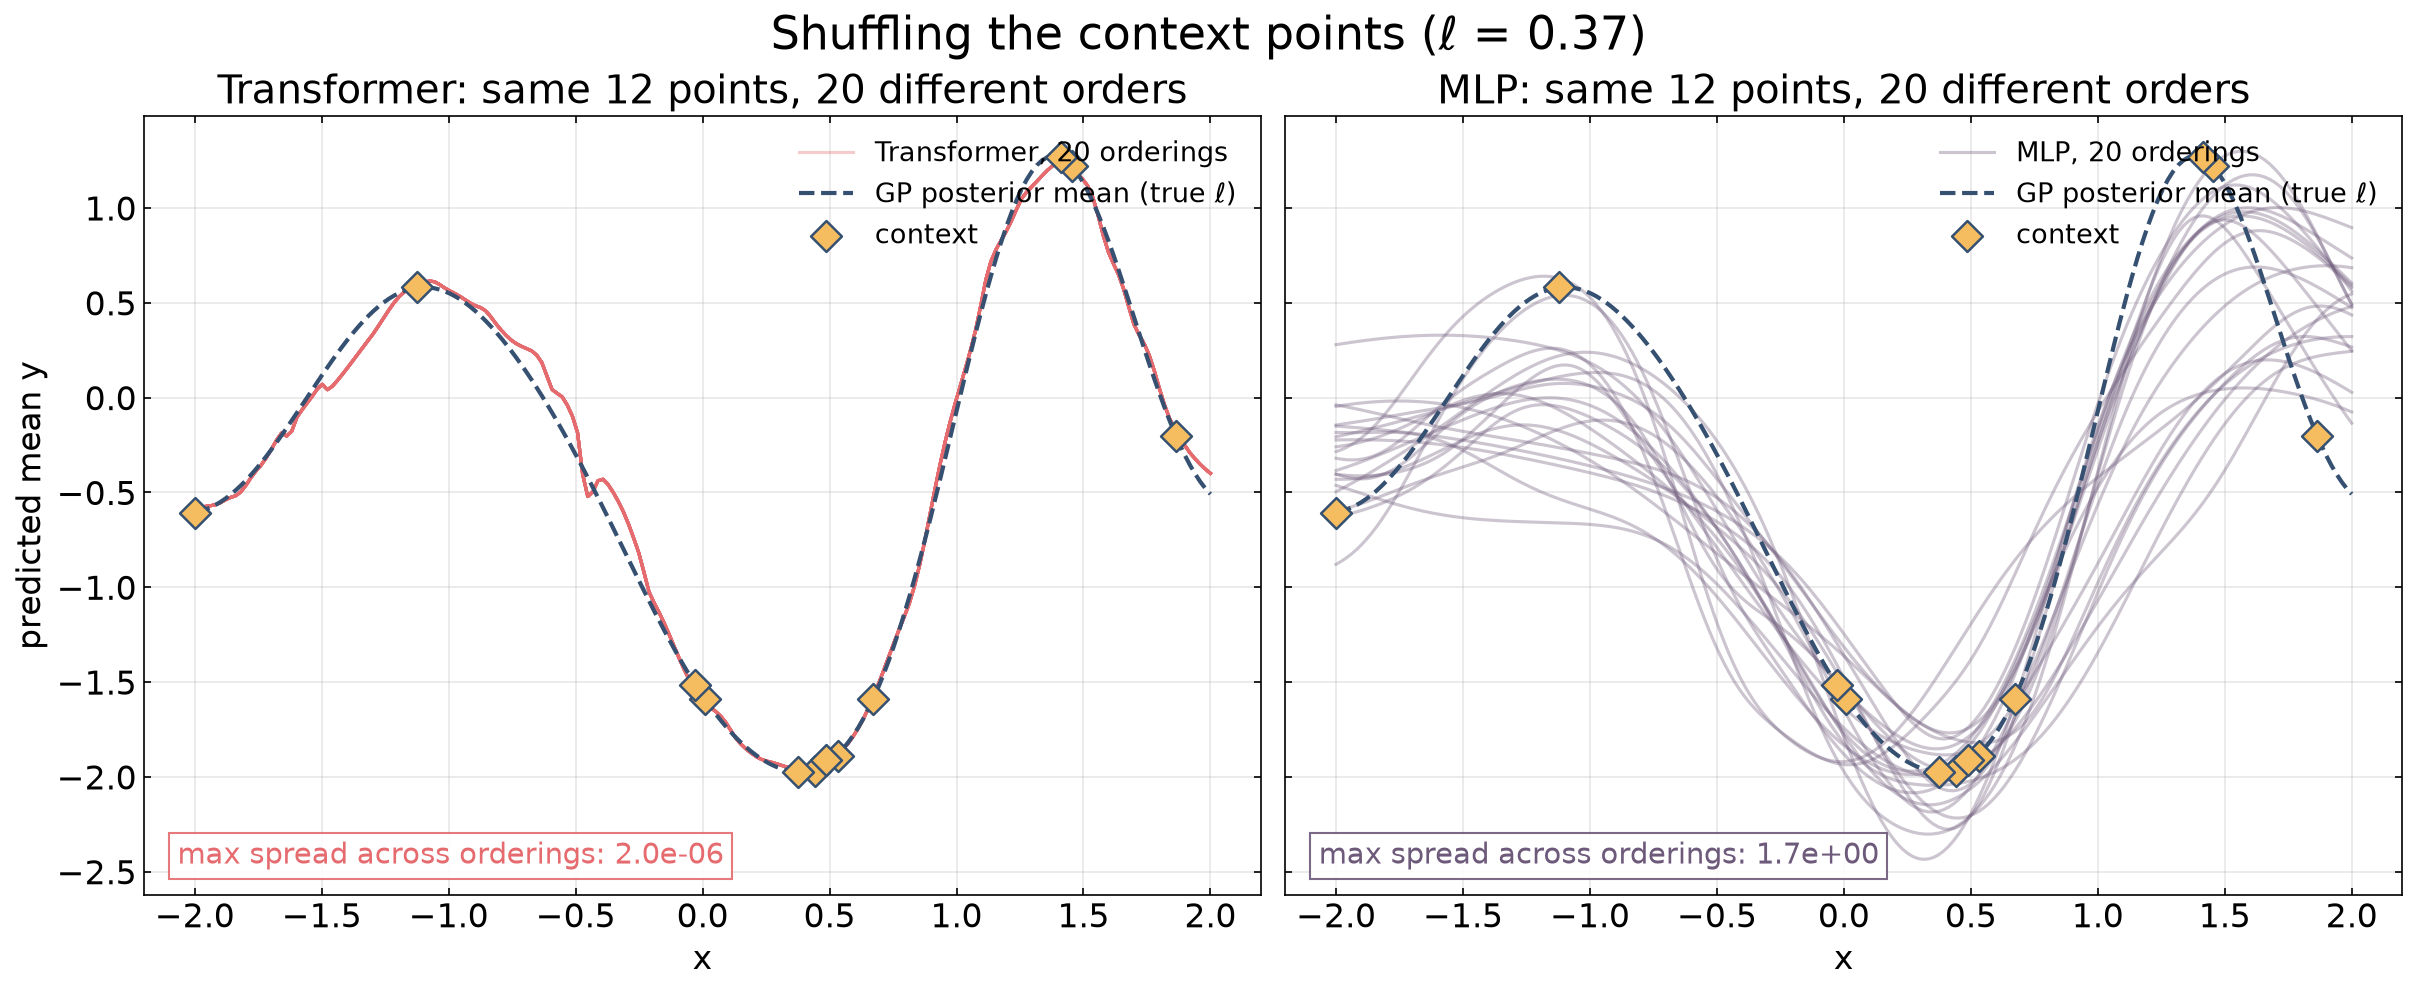
\includegraphics[width=\linewidth]{figures/shuffle_context.png}
  \caption{Predictions for one function with the same context points fed in 20 different orders: the
  transformer (left) and the MLP (right).}
\end{figure}

\section*{Additional plots}

\begin{figure}[H]
  \centering
  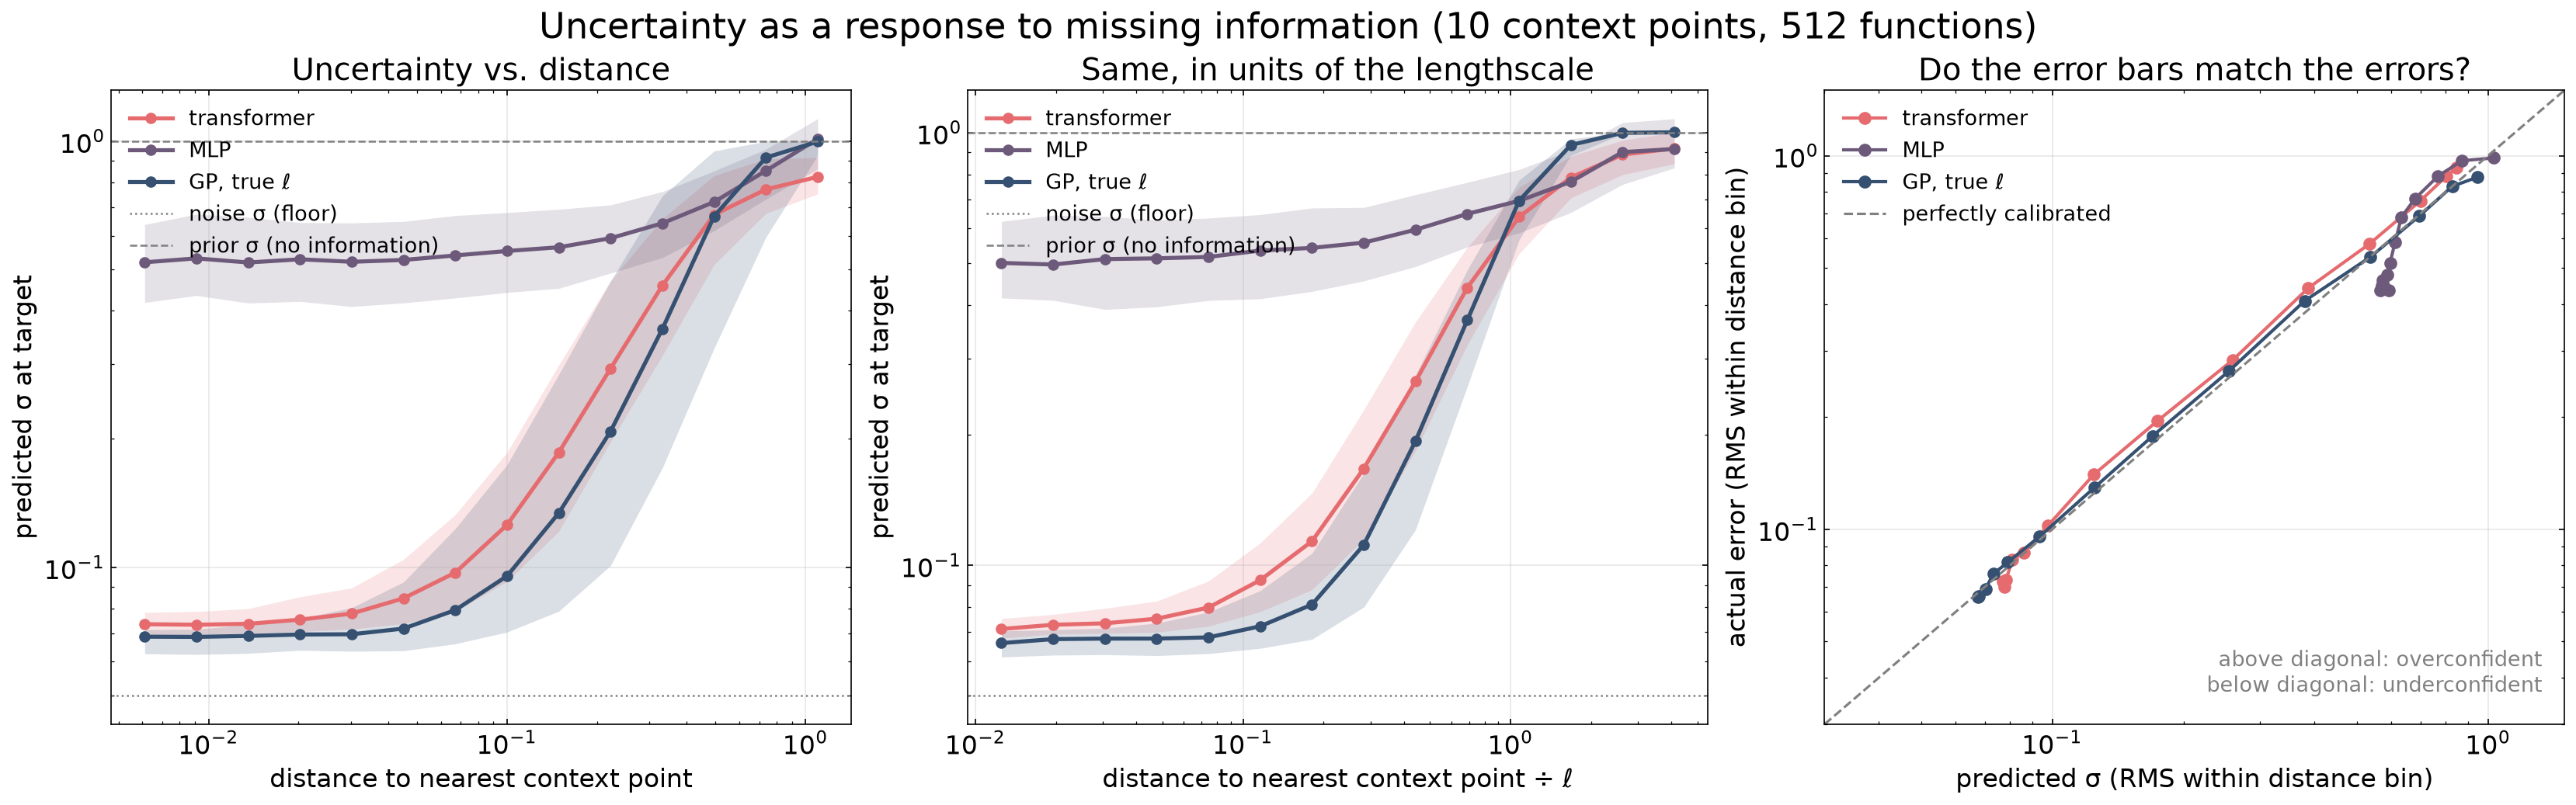
\includegraphics[width=\linewidth]{figures/uncertainty_vs_distance.png}
  \caption{Predicted uncertainty against distance to the nearest context point, in raw units (left) and in
  units of $\ell$ (middle), and predicted $\sigma$ against actual error (right).}
\end{figure}

\begin{figure}[H]
  \centering
  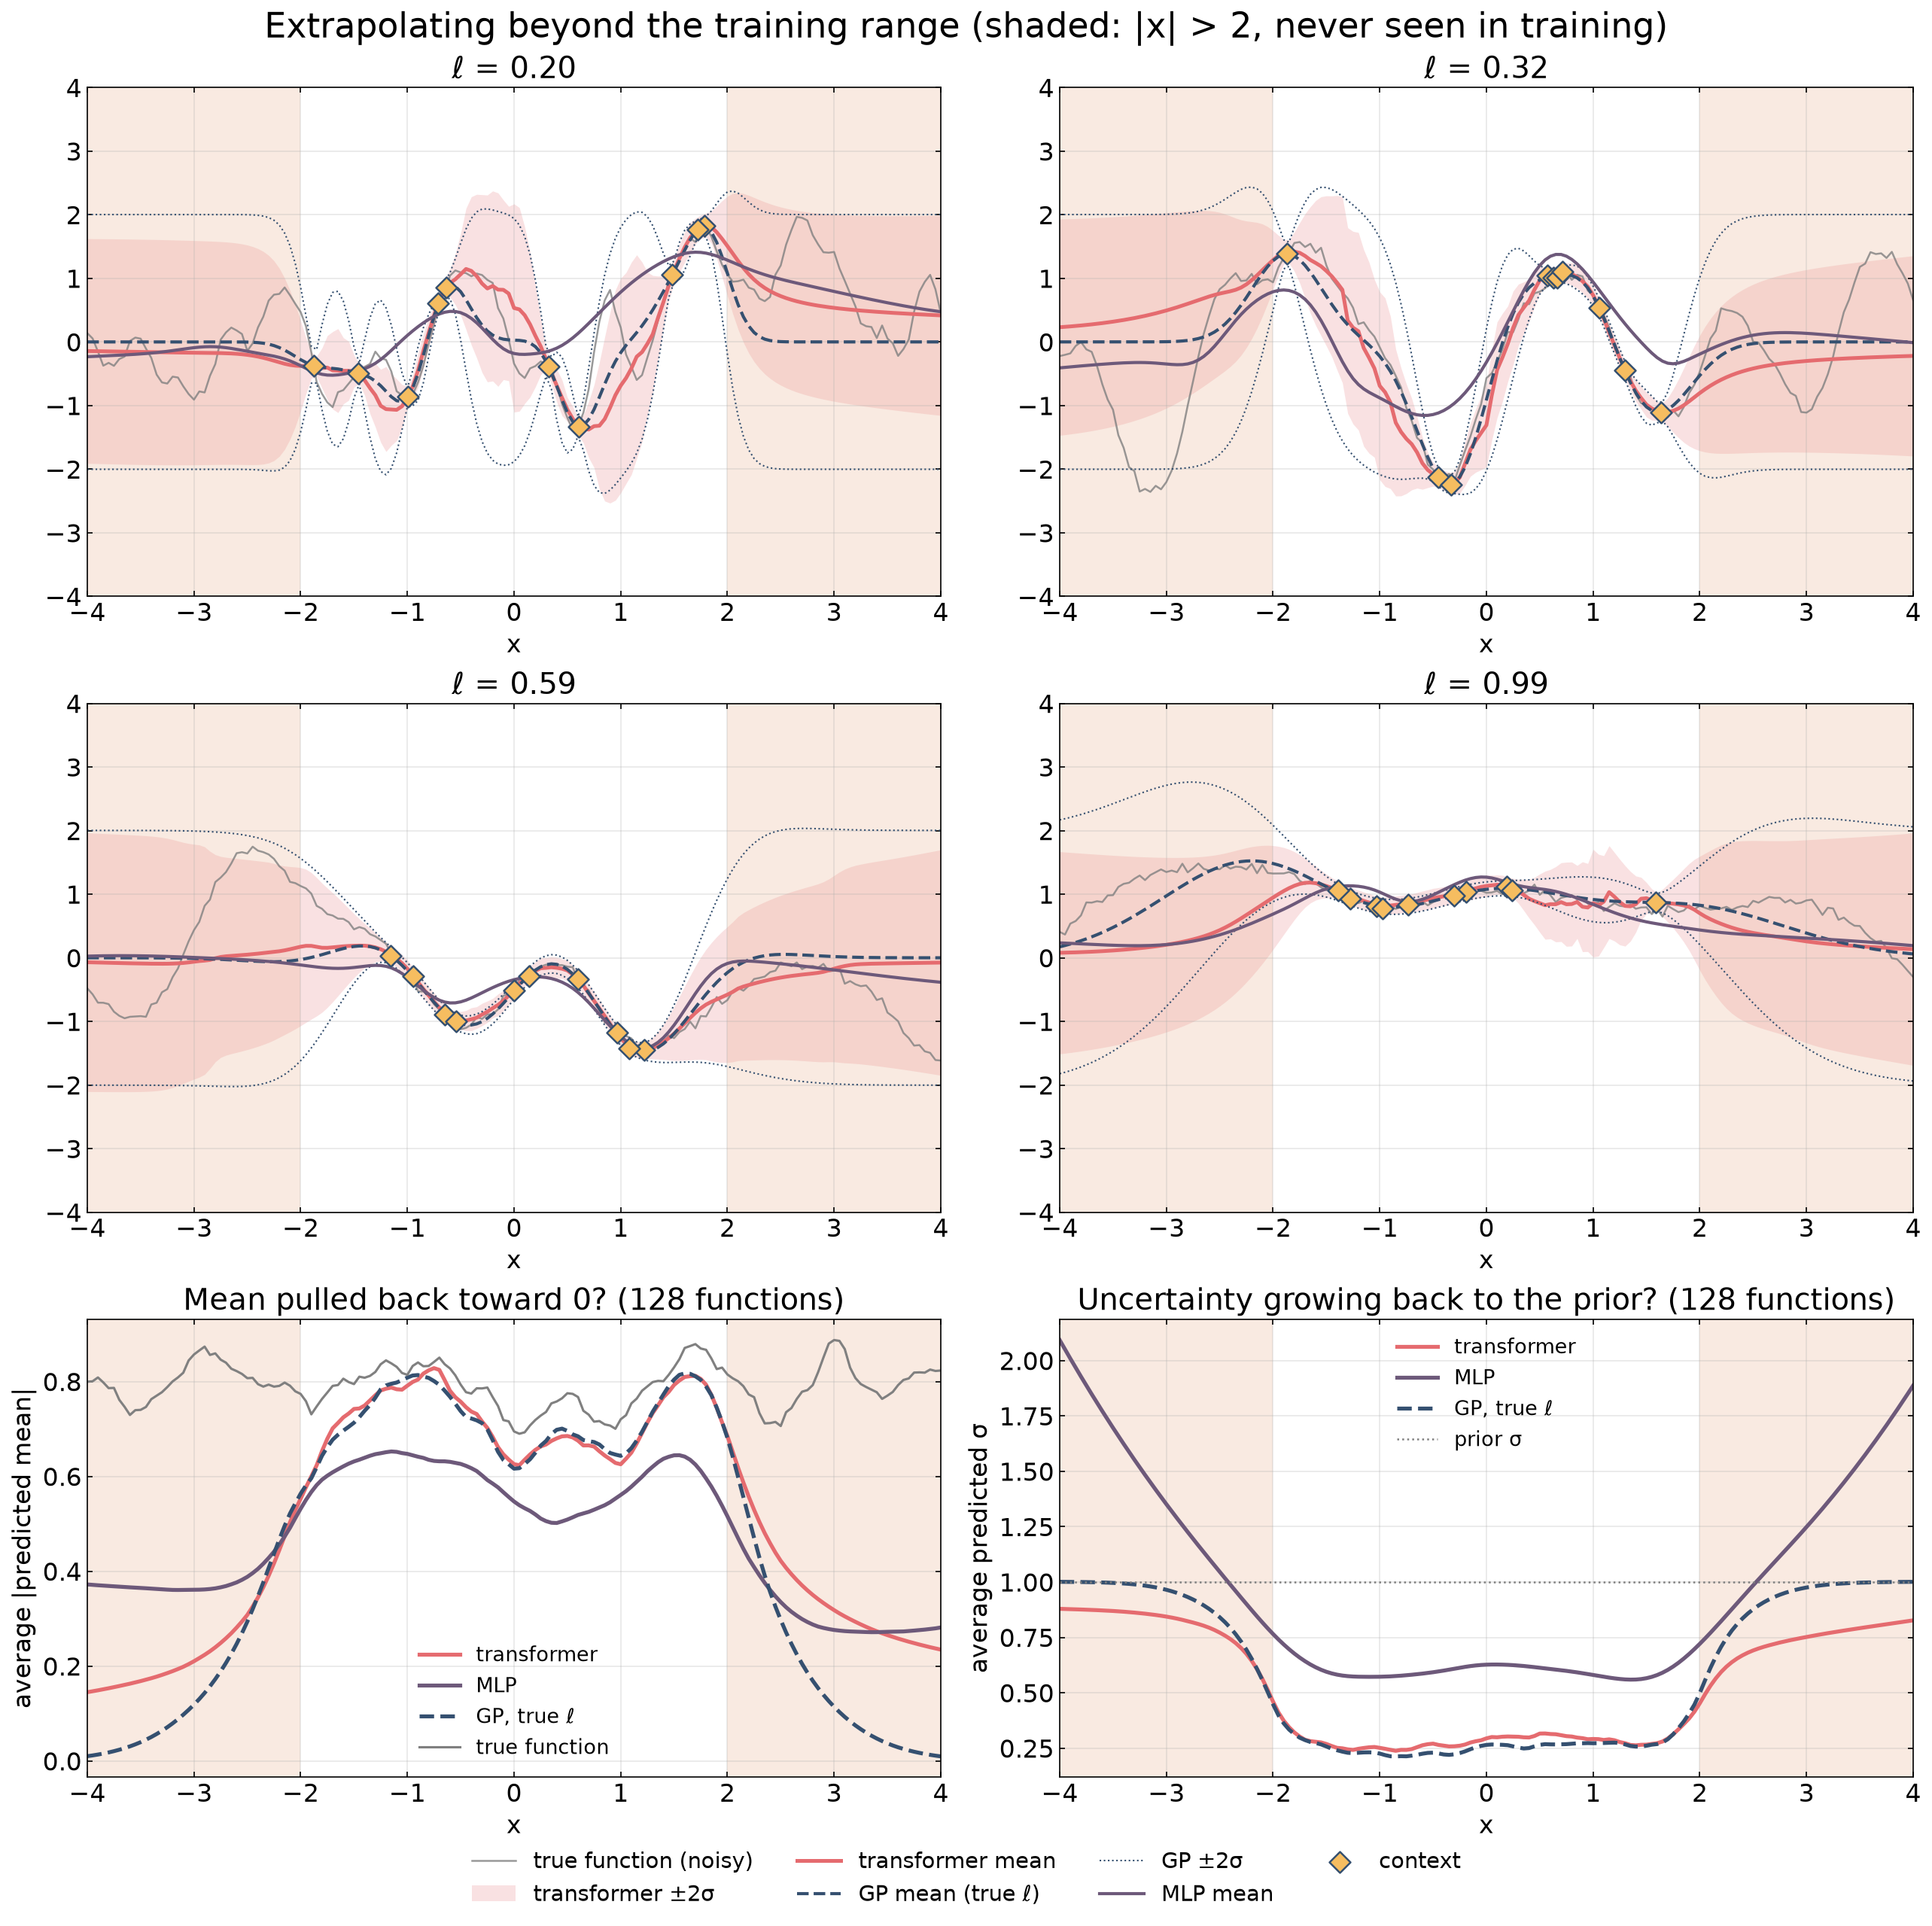
\includegraphics[width=0.85\linewidth]{figures/extrapolation.png}
  \caption{Predictions extrapolated to $x \in [-4, 4]$, beyond the training range $[-2, 2]$: four example
  functions, and the average $|$mean$|$ and $\sigma$ over 128 functions.}
\end{figure}

\end{document}
